\section{Experiments}
In this section, we evaluate the performance of our implementation on benchmark tasks. We begin by introducing the experimental settings. We then present the main results with runtime measurements. Finally, we conduct ablation studies for a fine-grained analysis of the acceleration.
% % \begin{table*}
%     [htbp]
%     \centering
%     \begin{minipage}[c]{0.58\linewidth}
%         \centering
%         \begin{tabular}{c|c|c|c}
%             Environment & Value               & Hyperparameter    & Value       \\
%             \hline
%             GPU         & NVIDIA A40          & Model             & LDM         \\
%             OS          & Ubuntu 22.04 Server & Dataset           & LSUN-Church \\
%             PyTorch     & 2.4.0               & Batch Size        & 32          \\
%             Python      & 3.11                & Timesteps         & 200         \\
%             CUDA        & 12.4.1              & Number of Samples & 128         \\
%         \end{tabular}
%         \caption{Benchmark Results for Model Performance Optimization}
%         \label{tab:hyper_table}
%     \end{minipage}
%     \hfill
%     \begin{minipage}[c]{0.38\linewidth}
%         \centering
%         \begin{tabular}{lccc}
%             \toprule \textbf{Mode} & \textbf{FID Score} & \textbf{Samples} \\
%             \midrule FP32          & 5.73               & 50000            \\
%             INT8                   & 5.85               & 50000            \\
%             INT4                   & 14.80              & 50000            \\
%             \bottomrule
%         \end{tabular}
%         \caption{FID Evaluation Results}
%         \label{tab:fid_eval}
%     \end{minipage}
% \end{table*}
\begin{table}
\begin{tabular}{lccc}
    \toprule \textbf{Mode} & \textbf{FID Score} & \textbf{Samples} \\
    \midrule FP32          & 5.73               & 50000            \\
    INT8                   & 5.85               & 50000            \\
    INT4                   & 14.80              & 50000            \\
    \bottomrule
\end{tabular}
\caption{FID Evaluation Results}
\label{tab:fid_eval}
\end{table}

\subsection{Experimental Settings}
\textbf{Dataset, Model, and Measurement.} We conduct experiments on the LSUN-Church-Outdoor dataset at a resolution of $256 \times 256$~\citep{yu15lsun}. For the model, we use a Latent Diffusion Model with a downsampling factor of 8, denoted LDM-8~\citep{rombach2022high}. We use the DDIM sampler with 200 sampling steps and $\eta = 0$~\citep{song2020denoising}. 
To assess the model's efficiency, we measure the runtime per generated sample and the DRAM transfer volume. We also report the Fr\'echet Inception Distance (FID)~\citep{heusel2017gans} evaluated on 50k generated images to assess the generation quality.

\textbf{Quantization Method.} We apply channel-wise static MSE quantization for the weights and dynamic tensor-wise quantization for the activations. To better handle activation outliers, we integrate SmoothQuant using training images from LSUN-Churches~\citep{xiao2023smoothquant}. 


% We utilize per-layer static quantization with per-output-channel weights and per-tensor activations. To handle activation outliers, we integrate SmoothQuant to migrate activation variance into the weights. 

\textbf{Hardware and Computation Platform.} We conduct experiments on an NVIDIA A40 GPU running Ubuntu 22.04 Server. Our software environment uses CUDA 12.4.1, Python 3.11, and PyTorch 2.4.0.


% The performance of the implementation was evaluated through benchmarking experiments using the environment settings and hyperparameters listed in Table~\ref{tab:hyper_table}.

\subsection{Main Results}
We generate 128 images with a batch size of 32 to evaluate runtime efficiency. Our experiments are conducted under FP32, INT8, and INT4 settings. For notational simplicity, we denote each configuration by its quantization method and precision. For instance, the method without modulated computation under INT8 precision is denoted as ``Baseline INT8'', while the method with modulated computation is denoted as ``MoDiff INT8''. We draw the following conclusions from the results.

\textbf{Running Time Speedup.} As shown in Table~\ref{tab:pipeline_speedup}, MoDiff achieves significant speedups over FP32 generation. Specifically, INT8-quantized generation with MoDiff achieved a speedup of 1.668$\times$, while INT4-quantized generation with MoDiff achieved a speedup of 1.800$\times$. It demonstrates the effectiveness of the optimizations and highlights MoDiff's potential to accelerate deep learning models.

% The performance of the implementation was compared with FP32 generation, INT8-quantized generation without MoDiff, and INT4-quantized generation without MoDiff. The results are presented in Table~\ref{tab:pipeline_speedup}. This benchmark demonstrates that the implementation achieves significant reductions in both computational cost and memory I/O.

% The results indicate that MoDiff with INT8 and INT4 quantization achieved significant speedups over FP32 generation. Specifically, INT8-quantized generation with MoDiff achieved a speedup of 1.668$\times$, while INT4-quantized generation with MoDiff achieved a speedup of 1.800$\times$. These findings demonstrate the effectiveness of the optimizations and highlight the potential of MoDiff for accelerating deep learning models.

\textbf{Efficient Memory Usage.} As shown in Table~\ref{tab:pipeline_speedup}, the DRAM transfer is substantially lower than that of FP32. For example, MoDiff INT4 uses only 66.7\% of the memory required by FP32. Although the DRAM transfer increases slightly relative to the baseline due to additional cache I/O, the overall memory savings remain promising.

\textbf{Generation Quality.} 
We evaluate the generation quality under different precision settings. With our kernels, the FID for FP32 is 5.73, for INT8 is 5.85, and for INT4 is 14.80. It shows that low-precision activations can still preserve generation quality, aligning with the results reported in the MoDiff paper.

% To assess whether the implementation meets the quality expectations of the original MoDiff, the quality of the generated images was evaluated using FID (Fr\'echet Inception Distance). The FID scores for FP32 generation, INT8-quantized generation with MoDiff, and INT4-quantized generation with MoDiff are reported in Table~\ref{tab:fid_eval}.

\subsection{Ablation Study}
We conduct ablation studies to provide a fine-grained analysis of the performance gains achieved by our kernels. We first partition the model into its individual components and evaluate the runtimes. We then investigate how different shapes affect the acceleration achieved in convolution.

% This section assesses the implementation's performance through systematic benchmarking, controlled experimental evaluation, and quantitative analysis. A comprehensive characterization of the computational cost of each model component is provided, supported by a rigorous theoretical examination of the corresponding performance metrics. The objective is to delineate the strengths and performance-limiting factors of the implementation, thereby yielding insights to inform and guide subsequent optimization efforts.
% \begin{figure*}[!ht]
    \centering
    \begin{subfigure}
        {0.58\textwidth}
        \centering
        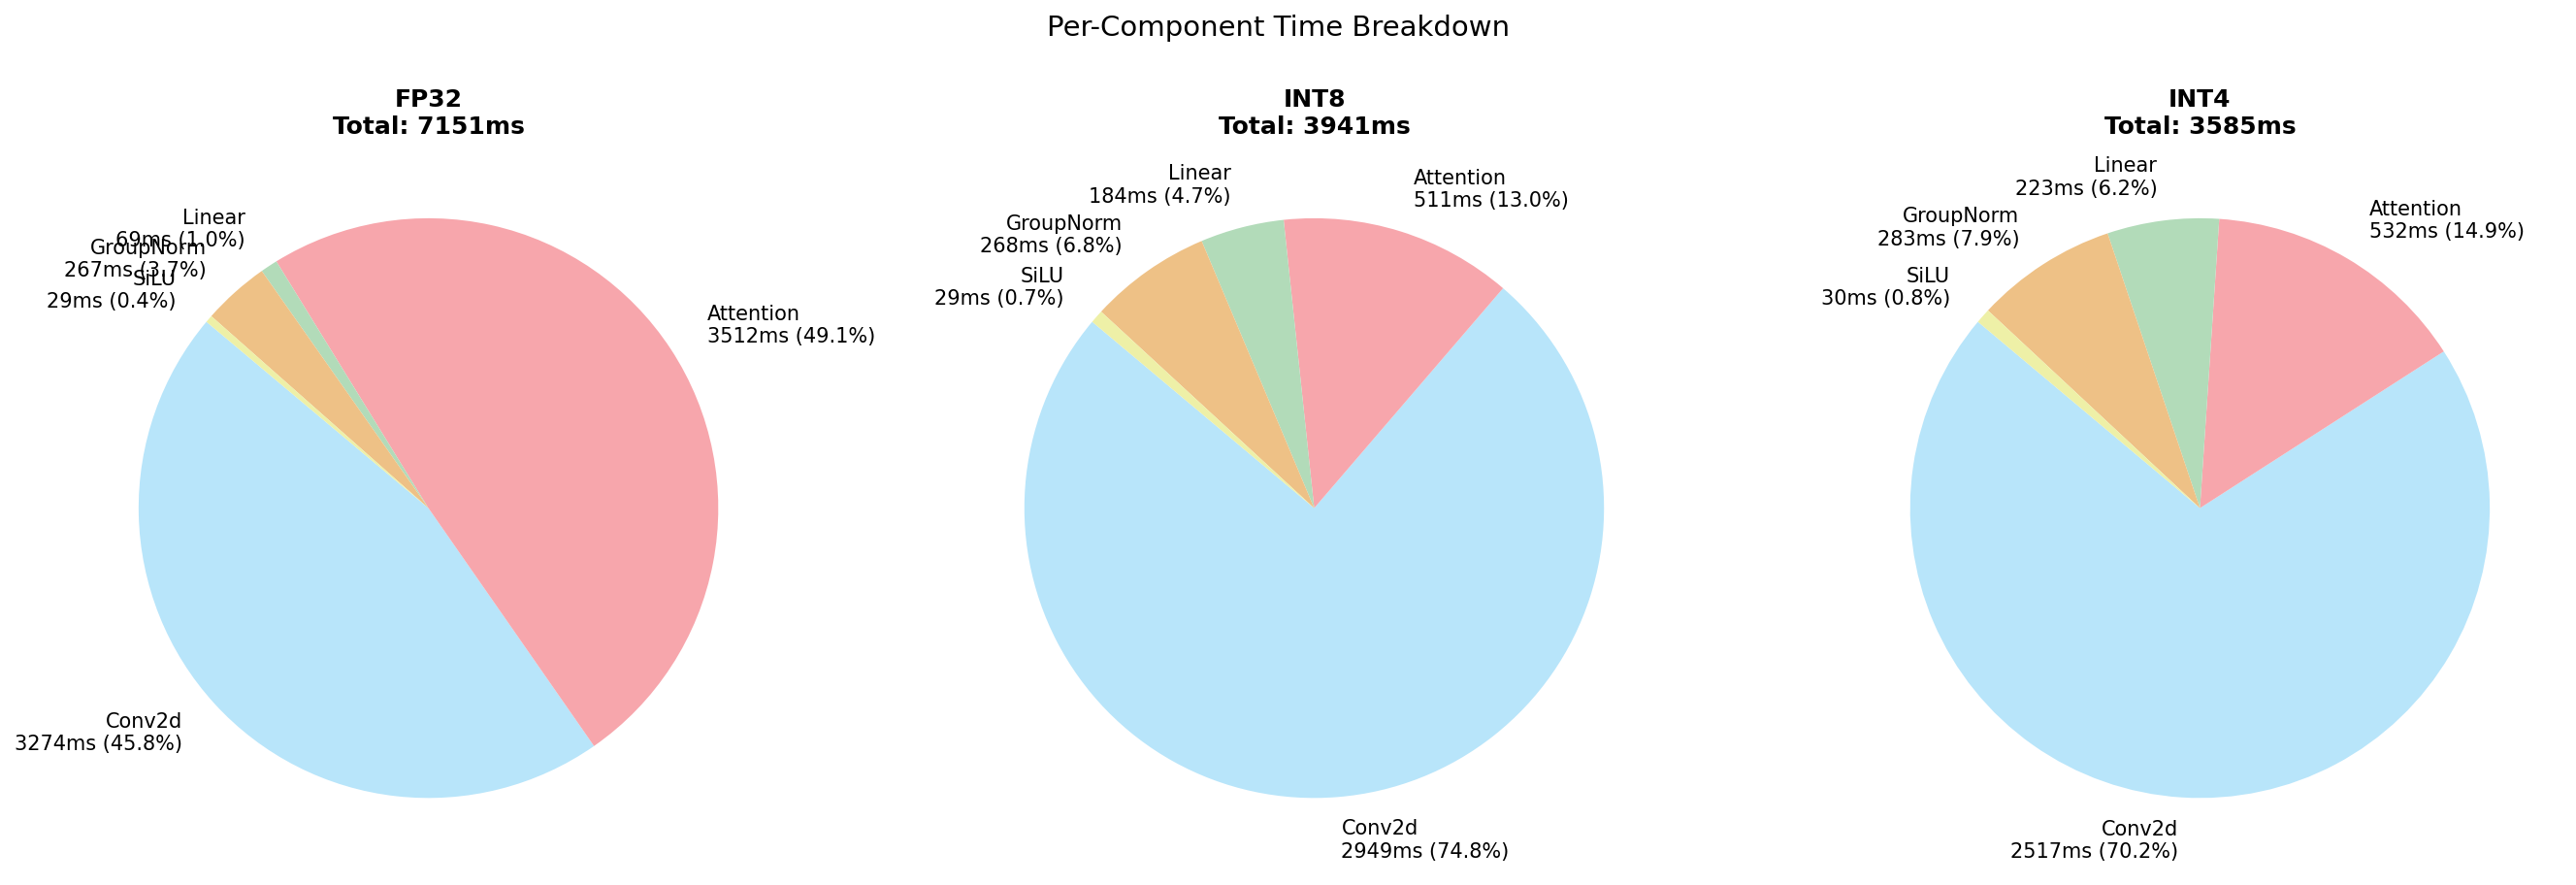
\includegraphics[width=\textwidth]{figures/plot_02_component_breakdown.png}
        \caption{Computational Cost Breakdown}
        \label{fig:plot_02}
    \end{subfigure}
    \hfill
    \begin{subfigure}
        {0.38\textwidth}
        \centering
        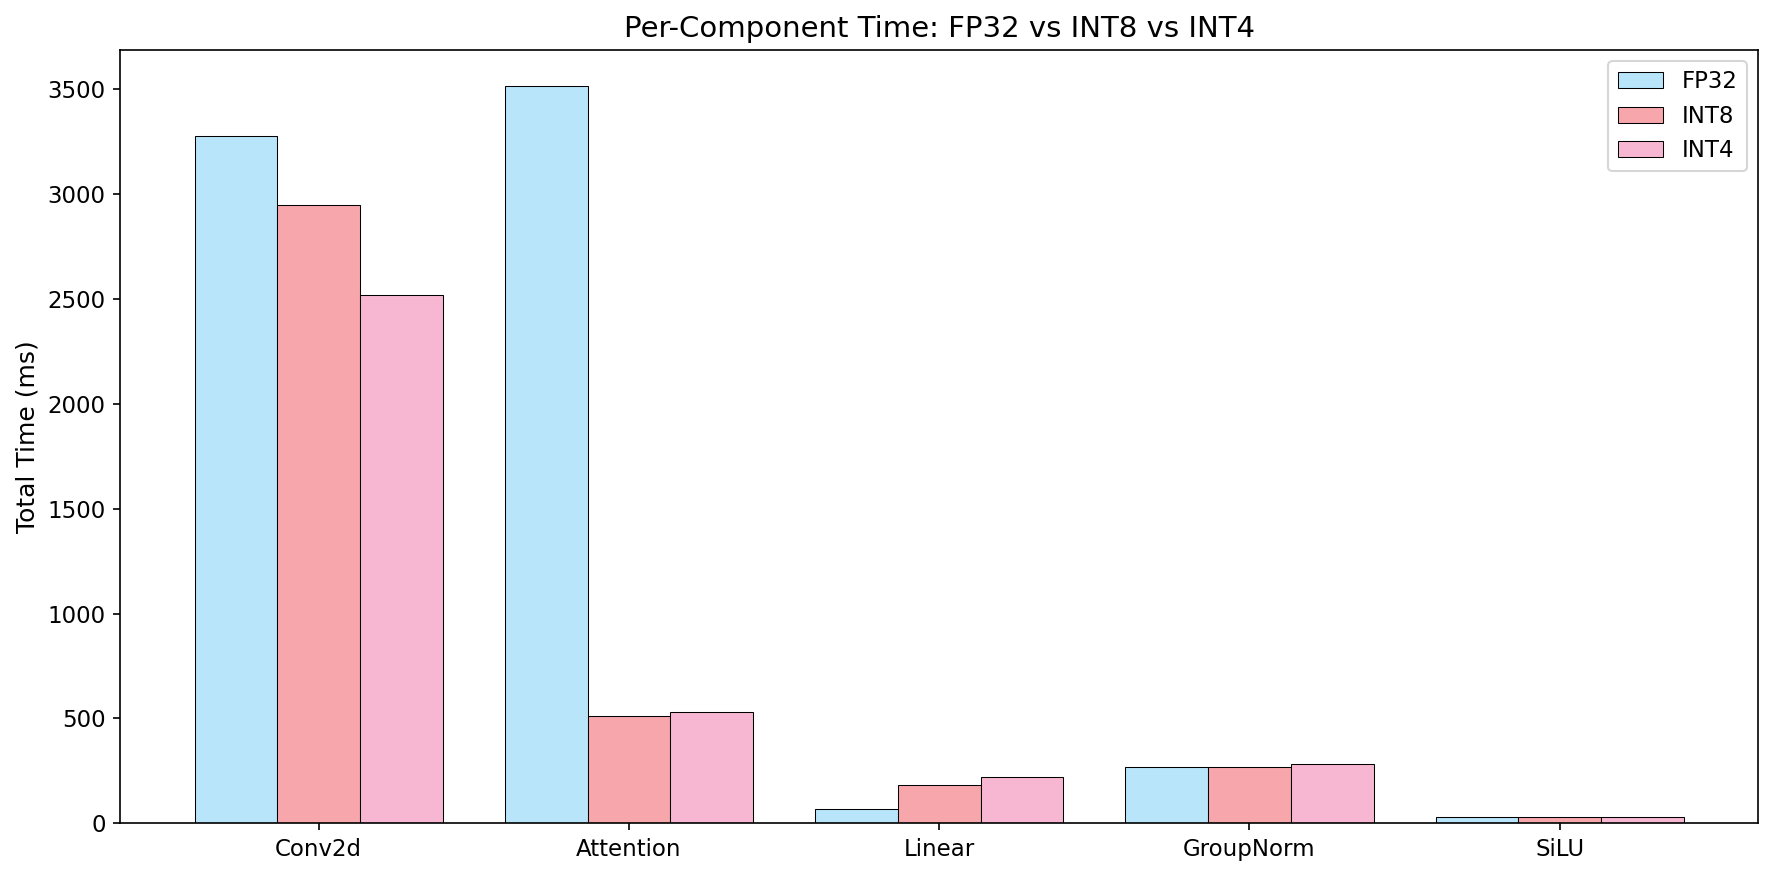
\includegraphics[width=\textwidth]{figures/plot_02b_component_bars.png}
        \caption{Computational Cost Breakdown (Bar Chart)}
        \label{fig:plot_02b}
    \end{subfigure}
    \caption{Computational Cost Breakdown}
    \label{fig:compu_cost_breakdown}
\end{figure*}
\begin{table}[t]
    \centering
    \caption{Component-wise time cost and speedup. The speedup is compared to FP32.}
    \label{tab:component_breakdown} \resizebox{\linewidth}{!}{
    \begin{tabular}{lr|rr|rr}
        \toprule Component & FP32   & INT8   &       Speedup       & INT4   &      Speedup        \\
        \midrule Conv2d    & 1410.0 & 1355.3 & 1.04$\times$ & 1126.3 & 1.26$\times$ \\
        Attention          & 1378.5 & 750.4  & 1.77$\times$ & 268.8  & 1.84$\times$ \\
        Linear             & 69.4   & 552.4  & 0.13$\times$ & 547.1  & 0.13$\times$ \\
        GroupNorm          & 7.5    & 7.7    & 0.98$\times$ & 60.1   & 1.00$\times$ \\
        SiLU               & 21.1   & 44.4   & 0.48$\times$ & 166.2  & 0.35$\times$ \\
        \bottomrule
    \end{tabular}}
\end{table}
\textbf{Computational Cost Breakdown.} As shown in Table~\ref{tab:component_breakdown}, most of the runtime accounts for the convolutional and linear layers. Our kernels reduce the runtime of both convolutional and linear layers. However, the remaining non-quantized layers still contribute significantly to the total computation, which explains why the overall optimization does not achieve the theoretical optimum.

% Component-level cumulative cost is detailed in Table~\ref{tab:component_breakdown} to identify where computational time is allocated.

% The detailed computational breakdown indicates that convolutional and attention layers are the primary contributors to the overall computational cost. This finding suggests that the MoDiff optimization, which reduces the time spent on convolutional operations, can substantially decrease the required computational resources. However, residual non-quantized layers continue to contribute significantly to the total computation, which accounts for the optimization's inability to achieve the theoretically optimal throughput of fully low-bit convolutional implementations.

\begin{table}[t]
    \centering
    \caption{Layer-wise speedup analysis across convolutional layers with different shapes. Here, \(C_{in}\) denotes the number of input channels, \(C_{out}\) denotes the number of output channels, and \(K\) denotes the kernel size. Count indicates how many times each layer shape appears in the model. The speedup is compared to FP32.}
    \label{tab:conv_layer} \resizebox{\linewidth}{!}{
    \begin{tabular}{lr|r|rr|rr}
        \toprule ($C_{in}$, $C_{out}$, K) & Count & FP32   & INT8   & Speedup      & INT4   & Speedup      \\
        \midrule (1536, 768, 3) & 5     & 0.3677 & 0.1452 & 2.53$\times$ & 0.0802 & 4.59$\times$ \\
        (768, 768, 3)           & 23    & 0.2220 & 0.0791 & 2.81$\times$ & 0.0439 & 5.06$\times$ \\
        (384, 384, 3)           & 21    & 0.1508 & 0.0518 & 2.91$\times$ & 0.0332 & 4.54$\times$ \\
        (192, 192, 3)           & 9     & 0.1434 & 0.0802 & 1.79$\times$ & 0.0479 & 2.99$\times$ \\
        (576, 192, 3)           & 1     & 0.0712 & 0.0654 & 1.09$\times$ & 0.0373 & 1.91$\times$ \\
        (768, 384, 1)           & 4     & 0.0370 & 0.0251 & 1.47$\times$ & 0.0218 & 1.70$\times$ \\
        (384, 192, 1)           & 2     & 0.0353 & 0.0228 & 1.55$\times$ & 0.0213 & 1.65$\times$ \\
        \bottomrule
    \end{tabular}}
\end{table}

\textbf{Layer-Wise Analysis.} To study the fine-grained acceleration behavior, we report the runtime for convolutional layers with different shapes. As shown in Table~\ref{tab:conv_layer}, most convolutional layers in LDM have a large number of channels. With these layers accounting for the majority of the computation, the achieved acceleration is substantial. The results demonstrate that our kernels provide significant improvements in computational efficiency.

% The CUTLASS-based convolution path and the efficiency of the fused kernels were evaluated by benchmarking representative U-Net convolution shapes; the results are summarized in Table~\ref{tab:conv_layer}. For most layers, INT8 yields a speedup of approximately $2\times$ to $3\times$, and INT4 achieves up to about $5\times$. The gains are smaller for certain $1\times1$ layers due to reduced arithmetic work and increased sensitivity to launch and quantization overhead. These results demonstrate that the kernels achieve significant improvements in computational efficiency.

% \begin{figure*}[!t]
    \centering
    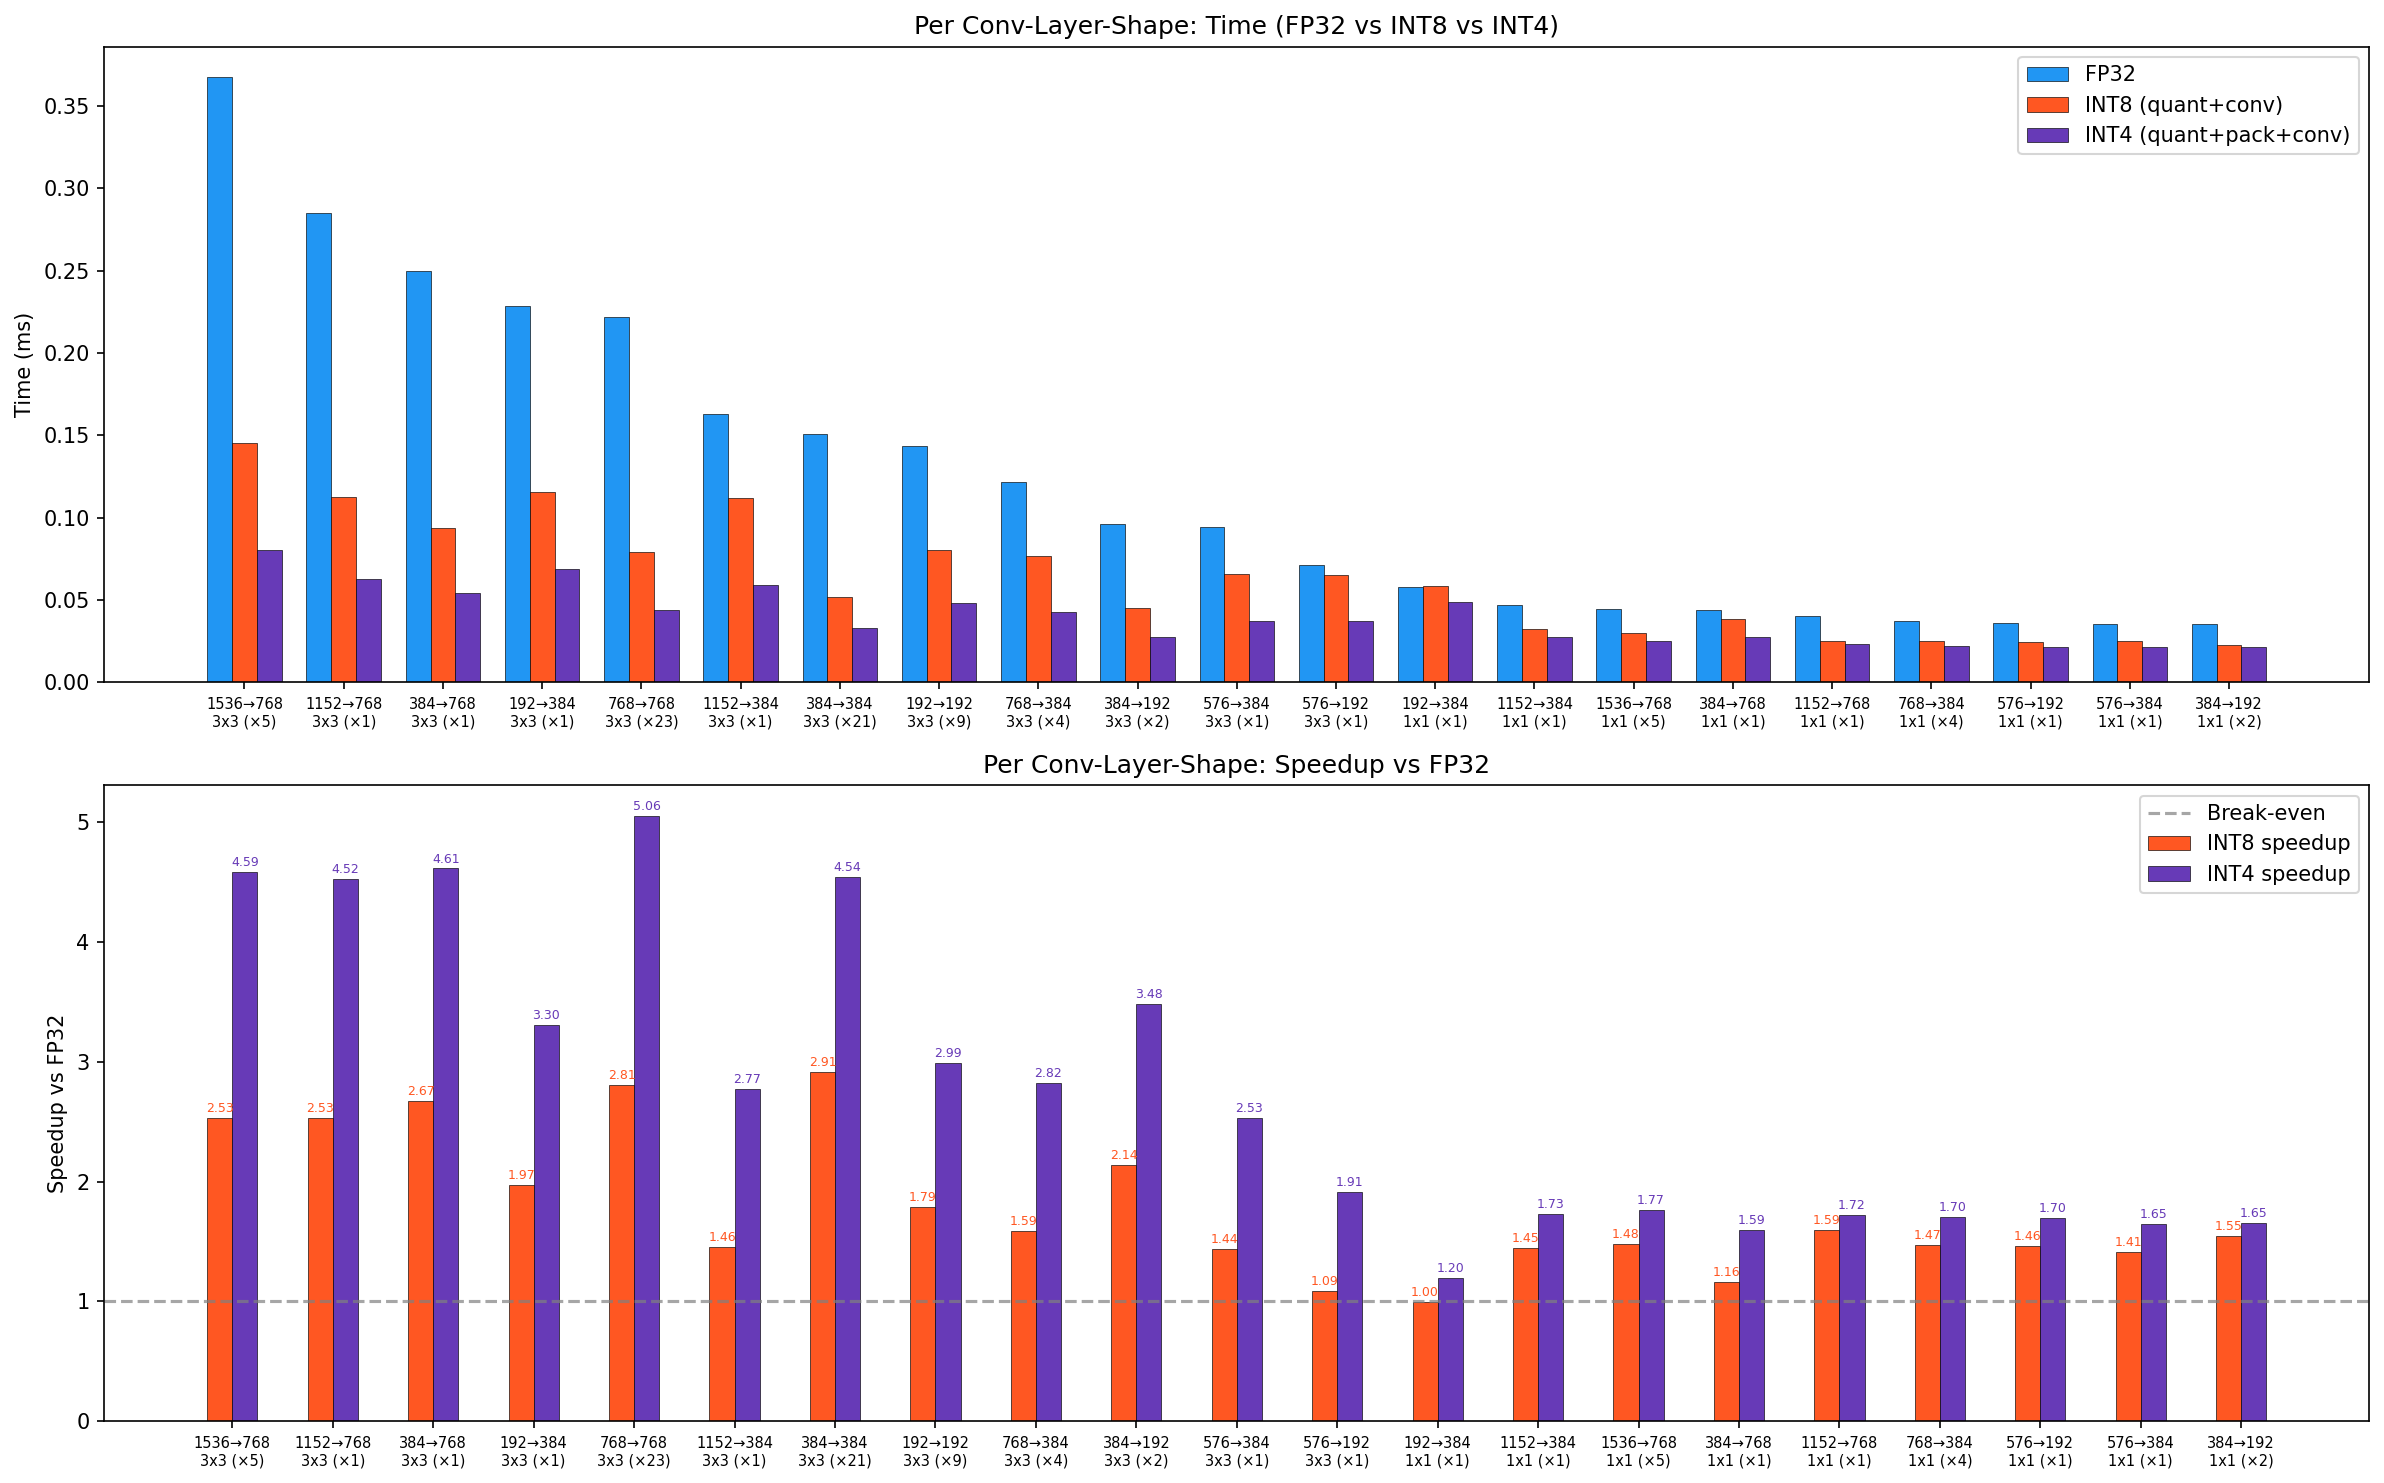
\includegraphics[width=0.80\textwidth]{figures/plot_03_conv_layer_analysis.png}
    \caption{Convolution-layer benchmark across representative UNet shapes.}
    \label{fig:plot_03_conv_layer_analysis}
\end{figure*}

% \subsection{Convolutional Layer Benchmark}

\subsection{Visualization}
We provide the visualization of the generated images in Fig.~\ref{fig:visualize_combined}. The results show that the low-bit quantization can still preserve the generation quality.
% \red{generated images}
\begin{figure}[t]
    \centering
    \begin{subfigure}
        [b]{0.325\linewidth}
        \centering
        
\includegraphics[width=\textwidth]{figures/comparison_results_seed42/image_fp32.png}
    \end{subfigure}
    \hfill
    \begin{subfigure}
        [b]{0.325\linewidth}
        \centering
        
\includegraphics[width=\textwidth]{figures/comparison_results_seed42/image_int8.png}
    \end{subfigure}
    \hfill
    \begin{subfigure}
        [b]{0.325\linewidth}
        \centering
        
\includegraphics[width=\textwidth]{figures/comparison_results_seed42/image_int4.png}
    \end{subfigure}
    \\
    \begin{subfigure}
        [b]{0.325\linewidth}
        \centering
        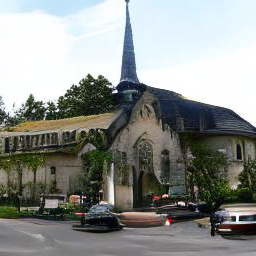
\includegraphics[width=\textwidth]{figures/comparison_results_seed128/image_fp32.png}
        \caption{FP32}
    \end{subfigure}
    \hfill
    \begin{subfigure}
        [b]{0.325\linewidth}
        \centering
        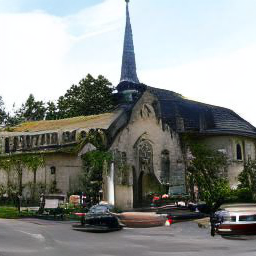
\includegraphics[width=\textwidth]{figures/comparison_results_seed128/image_int8.png}
        \caption{INT8}
    \end{subfigure}
    \hfill
    \begin{subfigure}
        [b]{0.325\linewidth}
        \centering
        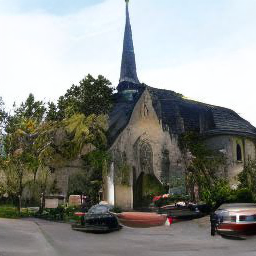
\includegraphics[width=\textwidth]{figures/comparison_results_seed128/image_int4.png}
        \caption{INT4}
    \end{subfigure}
    \caption{Generation Results Visualization.}
    \label{fig:visualize_combined}
\end{figure}
% \begin{figure}[t]
    \centering
    \begin{subfigure}
        [b]{0.31\linewidth}
        \centering
        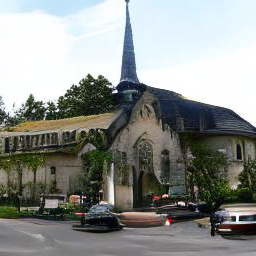
\includegraphics[width=\textwidth]{figures/comparison_results_seed128/image_fp32.png}
        \caption{FP32}
    \end{subfigure}
    \hfill
    \begin{subfigure}
        [b]{0.31\linewidth}
        \centering
        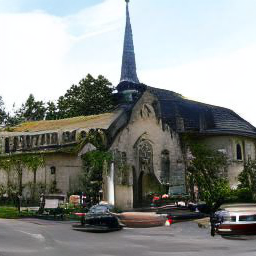
\includegraphics[width=\textwidth]{figures/comparison_results_seed128/image_int8.png}
        \caption{INT8}
    \end{subfigure}
    \hfill
    \begin{subfigure}
        [b]{0.31\linewidth}
        \centering
        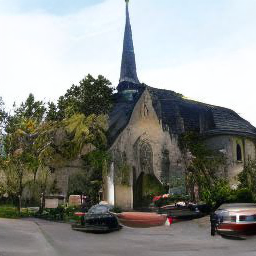
\includegraphics[width=\textwidth]{figures/comparison_results_seed128/image_int4.png}
        \caption{INT4}
    \end{subfigure}
    \caption{Comparison results visualization}
    \label{fig:visualize2}
\end{figure}